\clearpage
\twocolumn[{%
\rqparent
\subsection{The above-chance gate}
\label{app:rq00_gate_and_curves}

\noindent\begin{minipage}[t]{0.485\textwidth}
\vspace{0pt}
\paragraph{Research Question.} \emph{Which benchmarks clear chance at which size of the ladder, and which separate the language settings most?}

\paragraph{Setup.} We measure whether a benchmark task is above chance at a model size. We read the final checkpoints of the seed-1904 runs of every language setting, ladder and data build, 90M--1.7B. The tasks are every benchmark task with a chance level, in the languages the sweep trains. Per-language BPB and the bBPB twins have no chance level and are never gated. A run clears chance on a task when the one-sided 95 \% Wilson lower bound of its accuracy over the task's items is above the chance level. A (task, size) cell is above chance when at least half of the runs of that size that train the task's language clear it. We also apply the same rule to the benchmarks we screened, which were evaluated only on the final checkpoints of the larger models (Figure~\ref{fig:app_rq00_chance_considered} and Table~\ref{tab:app_rq00_pass_counts_considered}). On the tasks that clear chance at very small token counts of their language, we check which option the runs pick (Table~\ref{tab:app_rq00_early_passes}).
\end{minipage}\hfill
\begin{minipage}[t]{0.485\textwidth}
\vspace{0pt}
\begin{rqfinding}
\textbf{1. The gate removes most of the evaluation somewhere on the ladder.} On the 933 trained tasks, 377 (40 \%) are above chance at 90M and 599 (64 \%) at 1.7B. (Figure~\ref{fig:app_rq00_gate_and_curves}.)
\\
\\
\textbf{2. The picture is the same over all 1,696 tasks with a chance level.} Of the 1,511 scored at 90M, 619 (41 \%) pass, and 946 of 1,667 (57 \%) pass at 1.7B. 710 (42 \%) never pass, 29 of them because they are never scored.
\\
\\
\textbf{3. The answer format, more than the option count, decides the gate.} On the trained languages at 1.7B the letter-answer families nearly vanish while their cloze twins pass: \texttt{belebele} 3 / 59 tasks against 57 / 59, \texttt{global\_mmlu\_full} 1 / 29 against 29 / 29, \texttt{include\_base\_44} 3 / 36 against 29 / 36.
\end{rqfinding}
\end{minipage}

\vspace{\baselineskip}
\noindent\begin{minipage}{\textwidth}
\centering
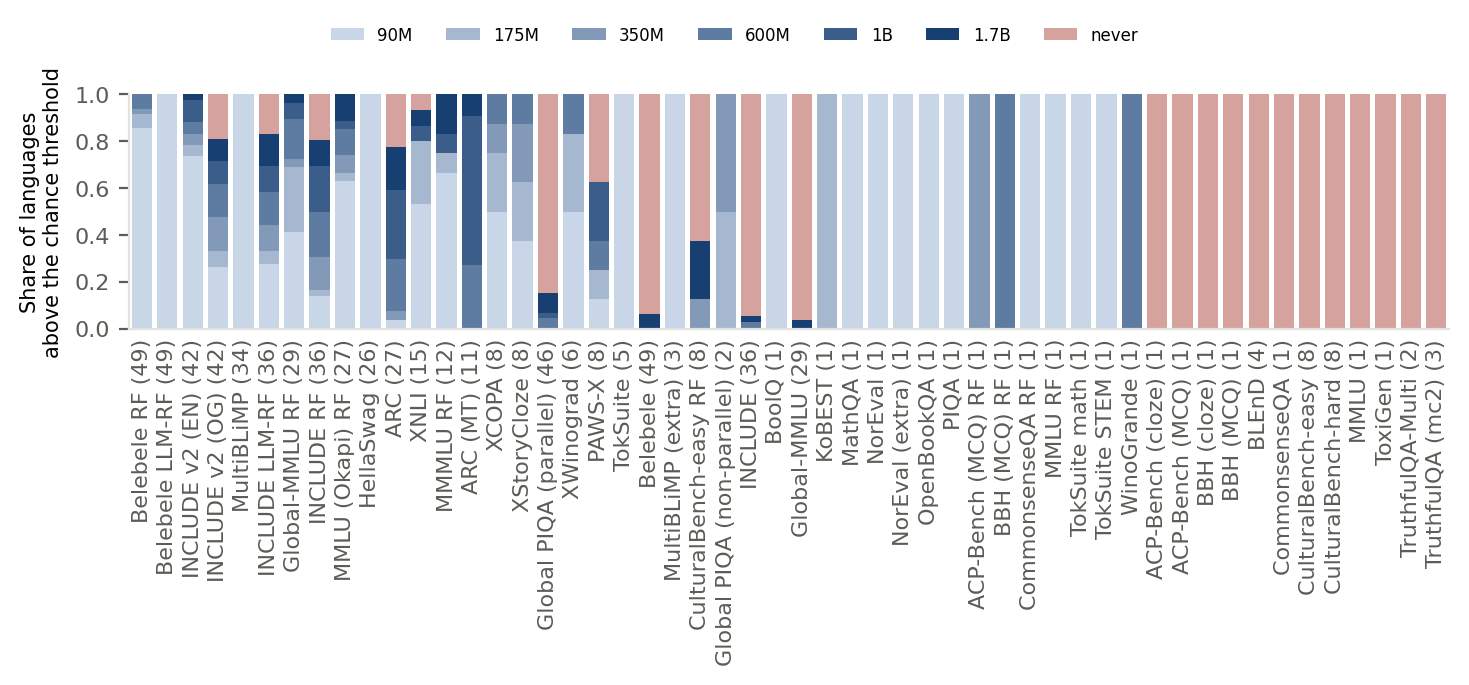
\includegraphics[width=\textwidth,height=0.36\textheight,keepaspectratio]{figures/app_rq00_chance_share_horizontal.png}
% source: src/signal-and-noise/analysis/rq00_gate_and_curves/pretraining/predictivity/first_size_share_paper_horizontal.png
\captionof{figure}{\textbf{The gate removes most of the evaluation somewhere on the ladder.} One bar per benchmark gives the share of its language tasks that clear the above-chance gate, split by the smallest model size from which the gate holds (a darker blue is a larger size). Red marks the tasks that stay at chance up to 1.7B. The number in parentheses is the benchmark's number of language tasks. The benchmarks are ordered from the most to the fewest tasks above chance.}
\label{fig:app_rq00_gate_and_curves}
\end{minipage}
}]

